%%%%%%%%%%%%%%%%%%%%%%%%%%%%%%%%%%%%%%%%%%%%%%%%%%%%%%%%%%%%%%%%%%%%%%
%%                     Domain
%%%%%%%%%%%%%%%%%%%%%%%%%%%%%%%%%%%%%%%%%%%%%%%%%%%%%%%%%%%%%%%%%%%%%%

\section{\glyph{Entity} nesting }
\label{sec:domain}

\SBGNERLone Version 2 allows \glyph{entities} to be nested. The enclosed \glyph{entity} represents a part of the enclosing \glyph{entity}, note that this relation between \glyph{entities} of different levels does not imply anything about \glyph{entities} of the same level. In the \fig{domain}, A is part of X and B is part of X. However, nothing is said about A and B. A and B could be of different nature (transmembrane domain and transduction domain) or could be overlapping (binding domain and catalytic domain sharing some amino-acids). 

\begin{figure}[H]
  \centering
  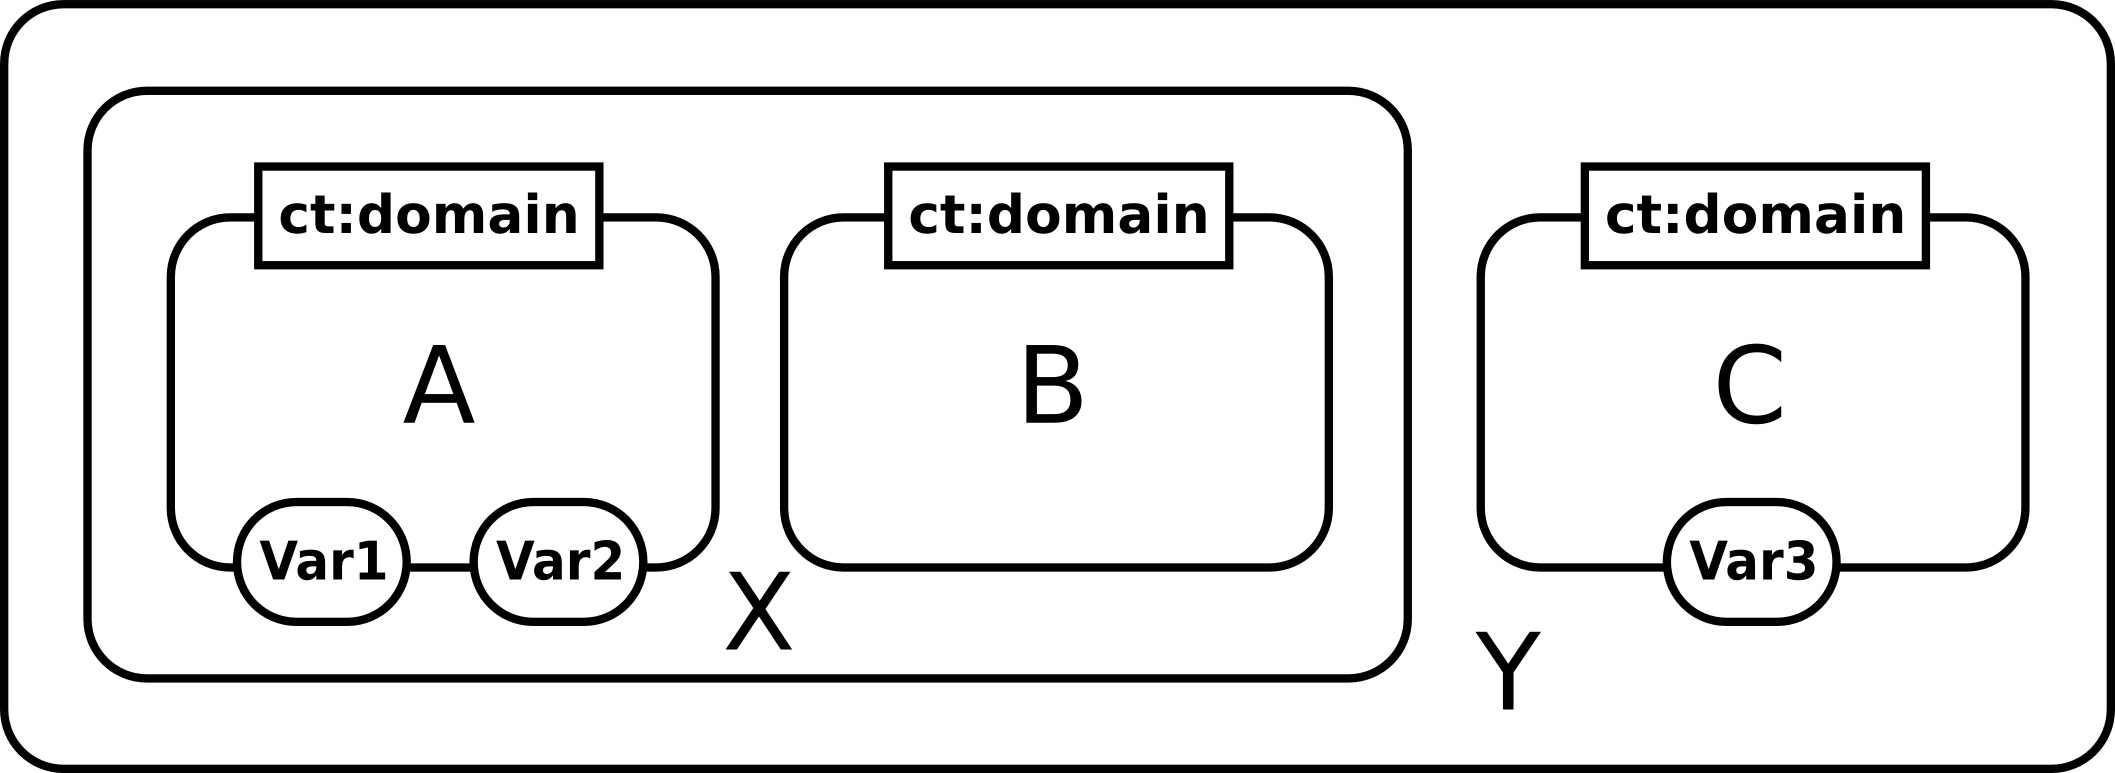
\includegraphics[scale = 0.3]{images/domain}
  \caption{The \ER glyph for \glyph{domain}.}
  \label{fig:domain}
\end{figure}

As any other \glyph{entity}, a nested \glyph{entity} can carry \glyph{state variables} and \glyph{units of information}. The contour of the containing \glyph{entity} must surround the totality of all contained \glyph{entities} including their \glyph{state variables} and \glyph{units of information}. This does not include the \glyph{assignments} and the \glyph{variable values}. A nested \glyph{entity} can participate in \glyph{interactions}, with ``sibling'' \glyph{entities} (part of the same containing \glyph{entity}), or others. They can also generate \glyph{influences}. For more information about the use and interpretation of entity nesting, see \sect{semanticsDomain} 

\begin{figure}[H]
  \centering
  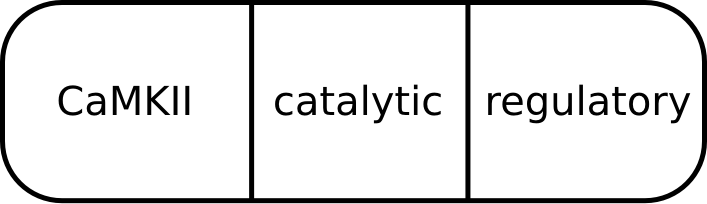
\includegraphics[scale = 0.5]{examples/ex-domain}
  \caption{Illustration of the use of \glyph{domains}. This map contains five \glyph{entities}. Three are top-level, while the \glyph{entities} ``res10-180'' and ``auto-inhibitory'' are domains of the \glyph{entity} ``CaMKII''. The controlled terms carried by the \glyph{units of information} tell us that those \glyph{domains} are a catalytic domain and a binding site respectively.	As far as the relationships with the \glyph{entities} ``calmoduline'' and ``target'' are concerned, the interpretation does not differ from the one we would derive from a map where all the \glyph{entities} would be entirely separated. However the regulation of localisation of ``CaMKII'' to the post-synaptic densite (PSD) by phosphorylation of threonine 286 also causes the localisation of ``res10-180'' and ``auto-inhibitory'', even if none carry the \glyph{state variables} involved.}
  \label{fig:ex-domain}
\end{figure}
